\PassOptionsToPackage{unicode=true}{hyperref} % options for packages loaded elsewhere
\PassOptionsToPackage{hyphens}{url}
%
\documentclass[12pt,english,]{article}
\usepackage{lmodern}
\usepackage{amssymb,amsmath}
\usepackage{ifxetex,ifluatex}
\usepackage{fixltx2e} % provides \textsubscript
\ifnum 0\ifxetex 1\fi\ifluatex 1\fi=0 % if pdftex
  \usepackage[T1]{fontenc}
  \usepackage[utf8]{inputenc}
  \usepackage{textcomp} % provides euro and other symbols
\else % if luatex or xelatex
  \usepackage{unicode-math}
  \defaultfontfeatures{Ligatures=TeX,Scale=MatchLowercase}
\fi
% use upquote if available, for straight quotes in verbatim environments
\IfFileExists{upquote.sty}{\usepackage{upquote}}{}
% use microtype if available
\IfFileExists{microtype.sty}{%
\usepackage[]{microtype}
\UseMicrotypeSet[protrusion]{basicmath} % disable protrusion for tt fonts
}{}
\usepackage{hyperref}
\hypersetup{
            pdfauthor={Minh Thang Cao},
            pdfborder={0 0 0},
            breaklinks=true}
\urlstyle{same}  % don't use monospace font for urls
\usepackage[margin=1in]{geometry}
\usepackage{graphicx,grffile}
\makeatletter
\def\maxwidth{\ifdim\Gin@nat@width>\linewidth\linewidth\else\Gin@nat@width\fi}
\def\maxheight{\ifdim\Gin@nat@height>\textheight\textheight\else\Gin@nat@height\fi}
\makeatother
% Scale images if necessary, so that they will not overflow the page
% margins by default, and it is still possible to overwrite the defaults
% using explicit options in \includegraphics[width, height, ...]{}
\setkeys{Gin}{width=\maxwidth,height=\maxheight,keepaspectratio}
\setlength{\emergencystretch}{3em}  % prevent overfull lines
\providecommand{\tightlist}{%
  \setlength{\itemsep}{0pt}\setlength{\parskip}{0pt}}
\setcounter{secnumdepth}{0}
% Redefines (sub)paragraphs to behave more like sections
\ifx\paragraph\undefined\else
\let\oldparagraph\paragraph
\renewcommand{\paragraph}[1]{\oldparagraph{#1}\mbox{}}
\fi
\ifx\subparagraph\undefined\else
\let\oldsubparagraph\subparagraph
\renewcommand{\subparagraph}[1]{\oldsubparagraph{#1}\mbox{}}
\fi

% set default figure placement to htbp
\makeatletter
\def\fps@figure{htbp}
\makeatother

\usepackage{float}
\usepackage{indentfirst}
\usepackage[T1]{fontenc}
\usepackage{amsmath}
\usepackage{url}
\usepackage{tikz}
\usepackage[T1]{fontenc}
\usepackage[boxruled,vlined]{algorithm2e}
\SetKwBlock{Else}{else}{endif;}
% \renewcommand{\thealgocf}{}
\newcommand{\pnt}[1]{{\scriptstyle#1}}
\let\origfigure\figure
\let\endorigfigure\endfigure
\renewenvironment{figure}[1][2] {
    \expandafter\origfigure\expandafter[H]
} {
    \endorigfigure
}
\usepackage{etoolbox}
\makeatletter
\providecommand{\subtitle}[1]{% add subtitle to \maketitle
  \apptocmd{\@title}{\par {\large #1 \par}}{}{}
}
\makeatother
\ifnum 0\ifxetex 1\fi\ifluatex 1\fi=0 % if pdftex
  \usepackage[shorthands=off,main=english]{babel}
\else
  % load polyglossia as late as possible as it *could* call bidi if RTL lang (e.g. Hebrew or Arabic)
  \usepackage{polyglossia}
  \setmainlanguage[]{english}
\fi

\title{\textbf{Project Report}\\
\Large{An Implementation Of:}}
\providecommand{\subtitle}[1]{}
\subtitle{A Simple Randomized \(O(n\,log\, n)\)--Time Closest-Pair\\
Algorithm in Doubling Metrics}
\author{Minh Thang Cao}
\date{10 July 2020}

\begin{document}
\maketitle

\hypertarget{introduction}{%
\section{\texorpdfstring{1
\enspace Introduction}{1 Introduction}}\label{introduction}}

Implementation of an algorithm helps us observe its efficiency and
behavior in practice. In this report, I will briefly explain each part
of the closest-pair doubling algorithm {[}1{]}, show the program's
implementation along with practical running time analysis, and some
implementation techniques I used. The theoretical information in this
report fully refers to the work of A. Maheshwari, W. Mulzer and M. Smid,
see {[}1{]}.

Given a metric space \((P,dist)\), with doubling dimension \(d\), whose
\(P\) is a set of \(n\) points. The closest pair of points is the two
points with the distance \(\delta_0\) that satisfies
\(dist(p_1, p_2) \geq \delta_0\) for any point \(p_1, p_2 \in P\). Also,
the doubling dimension \(d\) of a metric space indicates that for every
point \(p\) in \(P\) and every real number \(R > 0\), the
\(ball_P(p, R)\) can be covered by at most \(2^d\) balls in \(P\) of
radius \(R/2\), see {[}1, Section 2{]}. By using the definition and
properties of the doubling metric space and its doubling dimension, the
algorithm will find the closest-pair distance without the direct use of
the points' coordinates in \(O(n\,log\,n)\) time.

The closest-pair algorithm consists of three smaller parts:

\vspace{-2.5truemm}

\begin{quote}
\begin{enumerate}
\item Computing a separating annulus, denoted \textsc{SepAnn}$(S,n,d,\mu,c)$
\item The refinement of \textsc{SepAnn}$(S,n,d,\mu,c)$, denoted \textsc{SparseSepAnn}$(S,n,d,t)$
\item The main recursive closest-pair algorithm, denoted \textsc{ClosestPair}$(S,n,d)$
\end{enumerate}
\end{quote}

\vspace{-2truemm}

Throughout the paper, let:

\vspace{-2truemm}

\begin{quote}
\begin{itemize}
\item $(P, dist)$ be a finite metric space in which $P$ is the set of all points, and $dist$ is the function that calculate the distance between any two points
\item $d$ be the space's doubling dimension
\item $S$ be a non-empty subset of $P$
\end{itemize}
\end{quote}

\vspace{-2truemm}

\underline{\emph{\textbf{Note}}}: I will only mention about 2D points
because of the extremely high running time of the algorithm in the space
more than 3D (in which the doubling dimension is approximately at least
\boldmath\(log_221\) that gives us the base case with more than
3,000,000 points). \unboldmath

\newpage

\hypertarget{algorithm-1-computing-a-separating-annulus}{%
\section{\texorpdfstring{2 \enspace Algorithm 1: Computing a separating
annulus}{2 Algorithm 1: Computing a separating annulus}}\label{algorithm-1-computing-a-separating-annulus}}

An important part of the main closest-pair algorithm is finding a
separating annulus in the subset \(S\). I will briefly describe this
algorithm in the next subsection, due to A. Maheshwari, W. Mulzer and M.
Smid {[}1, Section 3.1{]}.

\hypertarget{the-mathrmspntepapntnnsndmuc-algorithm}{%
\subsection{\texorpdfstring{2.1 The
\(\mathrm{S\pnt{EP}A\pnt{NN}}(S,n,d,\mu,c)\)
algorithm}{2.1 The \textbackslash{}mathrm\{S\textbackslash{}pnt\{EP\}A\textbackslash{}pnt\{NN\}\}(S,n,d,\textbackslash{}mu,c) algorithm}}\label{the-mathrmspntepapntnnsndmuc-algorithm}}

In this section, \(\mu \ge1\) is a real constant number, \(c\) is
calculated based on \(\mu\) (I would say that \(c = 2(4\mu)^d\) {[}1,
Remark 1{]} since \(\mu\) is not an integer in this case {[}1, Section
3.2{]}).

This algorithm picks a uniformly random point \(p\) from the subset
\(S\) then finds the smallest ball centered at \(p\), denoted
\(ball_S(p, R_p)\), that contains at least \(n/c\) point. If the outer
ball \(ball_S(p,\mu R_p)\) contains at most \(n/2\) points, it returns
\(p\) and \(R_p\). If not, this procedure is repeated until the
condition is satisfied. This algorithm's pseudocode is given below, see
{[}1, Section 3.1{]}.

\begin{figure}[ht]
  \centering
  \begin{minipage}{0.9\linewidth}
    {\LinesNotNumbered
    \begin{algorithm}[H]
    \SetKwInOut{Input}{Input}
    \Input{Let $S$ be a subset of $P$, of size $n$, $d$ be the metric space's doubling dimension, $\mu \geq 1$ and $c >1$ be large enough real numbers. }

    \SetKwInOut{Output}{Output}
    \Output{A point $p \in S$ and a radius $R_p > 0$.}
    \DontPrintSemicolon
    \SetAlgoLined
    \BlankLine

    \centering
    \begin{minipage}{.80\linewidth}
    \Repeat{$|ball_S(p, \mu R_p)| \leq n/2$}
      {p = a uniformly random point in $S$;

      $R_p$ = min\{$r > 0: |ball_S(p, r)| \geq n/c$\};}
      return $p$ and $R_p$
    \end{minipage}
    \caption{\textsc{SparseSepAnn}$(S,n,d,t)$}
    \end{algorithm}}
  \end{minipage}
  \begin{minipage}{0.90\textwidth}
    \begin{flushright}
    {\footnotesize \emph{This pseudocode is from [1, Section 3.1]}\par}
    \end{flushright}
  \end{minipage}
\end{figure}

\hypertarget{finding-the-kth-smallest-element}{%
\subsection{\texorpdfstring{2.2 \enspace Finding the \(K^{th}\) smallest
element}{2.2 Finding the K\^{}\{th\} smallest element}}\label{finding-the-kth-smallest-element}}

One step in \textsc{SepAnn($S,n,d,\mu,c$)} algorithm is to find the
smallest ball which contains at least \(n/c\) points. This ball is easy
to find using the \(k^{th}\) smallest element algorithm. Particularly,
in a list of distances between \(p\) and all other points in \(S\), we
pick the \(\lceil n/c\rceil\)-th smallest element and let it be the
radius of the ball we need to find. Thus, all points closer to \(p\) are
inside this ball.

A very easy approach to find the \(k^{th}\) smallest element in a list
is to sort it in ascending order, and then simply return the element at
the \(k^{th}\) place. This sorting algorithm takes \(O(n\,log\,n)\) time
complexity in the worst case. Fortunately, we can improve the running
time to \(O(n)\) using a common recursive technique called QuickSelect,
which is similar to QuickSort.

Given an unordered list \(D\) which contains \(n\) numbers, and a
positive integer \(k\) satisfies \(1 \leq k \leq n\). Each element in
\(D\) has an index from \(0\) to \(n-1\). Consider a sublist of \(D\),
denoted \(D[a:b]\), which starts from index \(a\) and ends at \(b\),
inclusively. The base case is when \(a = b\), the algorithm returns the
only element in that sublist. If it is not the case, the algorithm will
choose a random \emph{pivot} in the list. The algorithm then rearranges
the list so that all elements smaller and larger than the pivot are to
the left and right of it, respectively. Now, the pivot has a new index,
says \(c\). If \(k = c-a+1\), the chosen pivot is the \(k^{th}\)
smallest element of \(D\), the algorithm returns \(D[c]\). If
\(k < c-a+1\), the algorithm recurses on the sublist to the left of the
pivot, \(D[a:c-1]\). If \(k > c-a+1\), the algorithm recurses on the
sublist to the right of the pivot, \(D[c+1:b]\). This algorithm's
pseudocode is given below.

\begin{figure}[ht]
  \centering
  \begin{minipage}{.9\linewidth}
    {\LinesNotNumbered
    \SetAlgoRefName{}
    \begin{algorithm}[H]
    \SetKwInOut{Input}{Input}
    \Input{Let $D$ be a list of double numbers, the integers $a$ and $b$ respectively be the starting and ending indices of a sublist and $k$ be an integer refers to the $k^{th}$ smallest element.}
    \SetKwInOut{Output}{Output}
    \Output{The $k^{th}$ smallest element in $D$, a double number.}
    \SetAlgoLined
    \BlankLine
    \centering
    \begin{minipage}{.75\linewidth}
        \uIf{$a == b$} {
            return $D[i]$
        }\Else {
      $p$ = a random element in $D$;
      
      \SetKwBlock{partitioning}{\textnormal{\textbf{rearranging:}}}{end;}

      \partitioning{
      all elements smaller than $p$ to the left of $p$;

      all elements larger than $p$ to the right of $p$;
      }

      
      $c$ = the current index of $p$ in $D$;

      \uIf{$k == c-a+1$} {
        return $p$
      }\uElseIf{$k < c-a+1$} {
        return \textsc{KthSmallest}$(D,a,c-1,k)$
      }\Else{
        return \textsc{KthSmallest}$(D,c+1,b,k)$
      }
    }
    \end{minipage}
    \caption{\textsc{KthSmallest}$(D, a, b, k)$}
    \end{algorithm}}
  \end{minipage}
\end{figure}

Unlike the original QuickSort algorithm, the QuickSelect recurses only
once and on one side after rearranging. This helps the algorithm remain
\(O(n)\) time complexity. By using the random selection, the pivot on
average is close to the middle of the list. Therefore, with the input is
an \(n\)-sized list \(D\), the recursive call is on a sublist whose size
is a half. Because the rearrangement takes \(O(n)\) time, this algorithm
takes at most \(2n\) time which is \(O(n)\). The running time is shown
below:

\[O(n) + O(n/2) + O(n/4) +... \leq O(2n) = O(n)\]

The following image is one of many outputs using different number of
elements and \(k\) value. I generated 100,000,000 numbers uniformly
random in the range {[}-100000, 100000{]} with \(k\) = 76,543,210.

\begin{figure}

{\centering 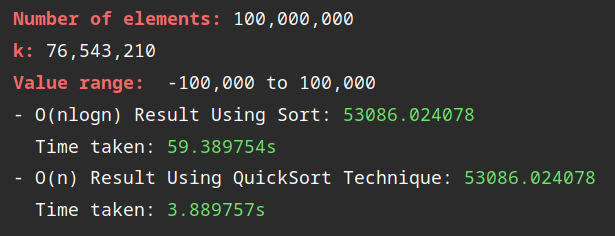
\includegraphics[width=0.7\linewidth]{./images_&_data/kth_smallest/100m} 

}

\caption{\label{fig1:figs}The outputs of the $O(NlogN)$ algorithm using regular sorting and the $O(n)$ QuickSelect algorithm that recurses only once.}\label{fig:unnamed-chunk-1}
\end{figure}

\hrule

~

~

With the given number of elements, \(k\) and value range, both of the
algorithms produced the same result, which is 53081.606002, but the
running times of them have a significant difference (For the program's
output, see Figure \ref{fig1:figs}).

Since the QuickSelect takes at most \(2n\) running time, the regular
sorting takes at least \(log(n)/2\) times more than it, and the \(log\)
is in base 2. In this case, there are 100,000,000 numbers, so:
\[\frac{log(n)}{2} = \frac{log(100,000,000)}{2} \approx 13.2877 \text{ times} \leq \frac{53.615235}{3.588446} \approx 14.9411 \text{ times}\]

Since \(14.9411\) is quite close to \(13.2877\), the running time of
this QuickSelect algorithm in practice is reasonable compared to the
theory.

\hypertarget{probability-to-select-a-good-point}{%
\subsection{2.3 Probability to select a ``good''
point}\label{probability-to-select-a-good-point}}

Again, the goal of algorithm \textsc{SepAnn($S,n,d,\mu,c$)} is to find a
``good'' point \(p\) in \(S\). A ``good'' point \(p\) implies that with
\(R_p\) (the radius of the smallest \(ball_S(p,R_p)\) that contains at
least \(n/c\) points), the \(ball_S(p,\mu R_p)\) contains at most
\(n/2\) points. Due to A. Maheshwari, W. Mulzer and M. Smid {[}1, Lemma
3{]}, the algorithm has probability at least \(1/c\) (about \(1/1623.4\)
in 2D space) to select a good point uniformly random from \(S\).

The number of times the algorithm \textsc{SepAnn($S,n,d,\mu,c$)} repeats
until it gets a good point depends on the way how the input points are
generated. I will show you some ways I use to generate the points based
on some patterns which produced different number of times the algorithm
repeats.

The first way is \textbf{generating uniformly random} points spread
throughout the space. This way of generating point produces a surprising
behavior of this algorithm. Every time \textsc{SepAnn($S,n,d,\mu,c$)} is
called, it only repeats \emph{once} until it gets to the base case, that
means the probability to get a good point is 100\%, see algorithm's data
on
\href{https://github.com/ThangMinhCao/closestpairdoubling/blob/master/report/Images/closest_pair/random_generation/random_sep_ann_data.txt}{\emph{GitHub
repository}}\footnote{Random points SepAnn data.
  \href{https://github.com/ThangMinhCao/closestpairdoubling/blob/master/report/images_\%26_data/closest_pair/random_generation/random_sep_ann_data.txt}{\emph{https://github.com/ThangMinhCao/closestpairdoubling/blob/master/rep-
  ort/images}\%\emph{26\_data/closest\_pair/random\_generation/random\_sep\_ann\_data.txt}}}.
Since the points are generated randomly, so they change every time,
there are no explanations about specific properties of the points in
this case. However, since \(100\%\) satisfied the probability at least
\(1/c\), this result is reasonable.

Another way is \textbf{generating points evenly in a grid}. Let \(n\) be
the number of points, \(a\) and \(b\) be any two factors of \(n\) that
satisfies \(a\times b = n\), \(d\) be the distances between any two
points which are close together. The points are set into the
\(a \times b\) grid which means each point is on a corner of a
\(d\)-sided square, see Figure \ref{fig:grid}.

\begin{figure}[!h]
\centering
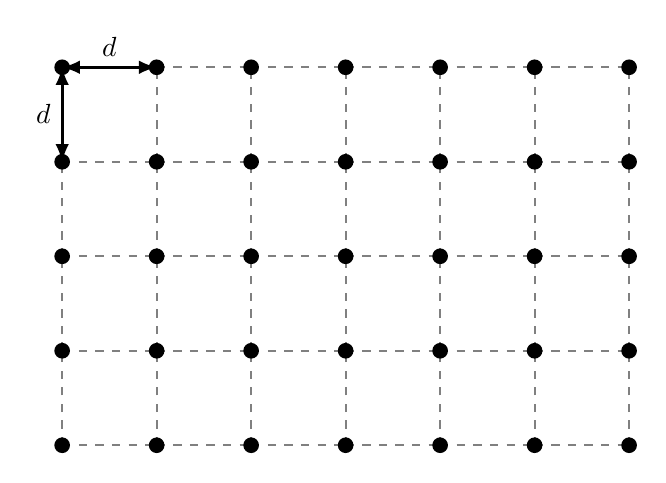
\begin{tikzpicture}
  \foreach \x in {0, 1, 2, 3, 4, 5, 6} {
    \foreach \y in {0, 1, 2, 3, 4} {
      \node (thisNode) at (1.2*\x, 1.2*\y) {};
      \ifthenelse{\x=6}{}{\draw[dashed,gray,thick] (1.2*\x, 1.2*\y) -- (1.2*\x+1.2, 1.2*\y);}
      \ifthenelse{\y=4}{}{\draw[dashed,gray,thick] (1.2*\x, 1.2*\y) -- (1.2*\x, 1.2*\y+1.2);}
      \node at (thisNode) [circle,fill=black,inner sep=2pt] {};
    }
  }
  \draw[black,very thick,latex-latex] (0, 1.2*4) -- node[above] {$d$} (1.2, 1.2*4);
  \draw[black,very thick,latex-latex] (0, 1.2*4) -- node[left] {$d$} (0, 1.2*3);
\end{tikzpicture}

\caption{An example of generating points in grid. A set of 35 points that gives us a $5\times7$ grid. Points are placed at corners of the squares with side is $d$ which could be any number.}
\label{fig:grid}
\end{figure}

\hrule

~

~

When using this grid way to generate points, the algorithm
\textsc{SepAnn($S,n,d,\mu,c$)} now repeats multiple times which is its
expected behavior, see. Again, the lowest probability in most of trials
in this case is about \(1/20\) which satisfies probability at least
\(1/c\), see Figure \ref{fig:data}. For the full grid input data, see
the
\href{https://github.com/ThangMinhCao/closestpairdoubling/blob/master/report/images_\%26_data/closest_pair/grid_generation/grid_sepann_data.txt}{\emph{GitHub
repository}}\footnote{Grid points SepAnn data.
  \href{https://github.com/ThangMinhCao/closestpairdoubling/blob/master/report/images_\%26_data/closest_pair/grid_generation/grid_sepann_data.txt}{\emph{https://github.com/ThangMinhCao/closestpairdoubling/blob/master/report/-}
  \emph{images}\%\emph{26\_data/closest\_pair/grid\_generation/grid\_sepann\_data.txt}}}.

\begin{figure}
\begin{minipage}{0.48\textwidth}
  \centering
  \begin{tabular}{|c|c|}
  \hline
  $\pmb n$   & \textbf{Repeat times} \\ \hline
   200000  & 6            \\ \hline
   193836  & 7            \\ \hline
   179534  & 2            \\ \hline
   172501  & 1            \\ \hline
   158381  & 13            \\ \hline
   156531  & 3            \\ \hline
  \ldots   & \ldots       \\ \hline
  \end{tabular}
\end{minipage}
\begin{minipage}{0.48\textwidth}
  \centering
  \begin{tabular}{|c|c|}
  \hline
  $\pmb n$   & \textbf{Repeat times} \\ \hline
  \ldots   & \ldots       \\ \hline
  101943   & 4            \\ \hline
   96367   & 2            \\ \hline
   96154   & 2            \\ \hline
   83621   & 6            \\ \hline
   83288   & 13           \\ \hline
   82515   & 2            \\ \hline
  \end{tabular}
\end{minipage}
\caption[Caption]{Given an input of 700,000 points generated in a grid. This is a portion of the data about the number of times the algorithm \textsc{SepAnn$(S,n,d,\mu,c)$} repeats.}
\label{fig:data}

\end{figure}

\hypertarget{algorithm-2-the-refinement-of-mathrmspntepapntnnsndmuc}{%
\section{\texorpdfstring{3 \enspace Algorithm 2: The refinement of
\(\mathrm{S\pnt{EP}A\pnt{NN}}(S,n,d,\mu,c)\)}{3 Algorithm 2: The refinement of \textbackslash{}mathrm\{S\textbackslash{}pnt\{EP\}A\textbackslash{}pnt\{NN\}\}(S,n,d,\textbackslash{}mu,c)}}\label{algorithm-2-the-refinement-of-mathrmspntepapntnnsndmuc}}

With the use of the algorithm \textsc{SepAnn$(S,n,d,\mu,c)$}'s output,
this refinement algorithm continues to find an annulus that separates
the points in \(S\) into different smaller sets of points.

Let \(\mu = e\) and \(c = 2(4e)^d\), see {[}1, Remark 1{]}. The
algorithm \textsc{SepAnn$(S,n,d,e,c)$} returns an annulus's center
\(p \in S\) and its radius, \(R'>0\). An input of this refined algorithm
is \(t > 0\), a large enough constant calculated based on \(n\). Let
\(R_i = (1+1/t)^i\cdot R'\), in which \(i\) is a uniformly random
element inclusively from \(1\) to \(t\). The algorithm then finds an
annulus centered at \(p\) with the inner radius \(R_{i-1}\) and outer
radius \(R_{i}\), denoted \(A_i = annulus_S(p, R_{i-1}, R_i)\). If the
annulus contains at most \(n/t\) points then we are done. The algorithm
returns \(p\) and \(R_{i-1}\). Otherwise, the previous procedure is
repeated until the condition is satisfied. The pseudocode of this
refined algorithm is given below, see {[}1, Section 3.2{]}.

\begin{figure}[ht] \centering
  \begin{minipage}{1\linewidth}
    {\LinesNotNumbered
    \begin{algorithm}[H]
    \SetKwInOut{Input}{Input}
    \Input{Let $S$ be a subset of $P$, of size $n \geq 2(4e)^d +1$, $d$ be the space's doubling dimension, $t \geq1$ be an integer.}
    \SetAlgoLined
    \SetKwInOut{Output}{Output}
    \Output{A point $p \in S$ and a radius $R > 0$.}
    \BlankLine

    \centering
    \begin{minipage}{.80\linewidth}
    $c = 2(4e)^d$;

    let $p\in S$ and $R' > 0$ be the output of algorithm \textsc{SepAnn$(S,n,d,e,c)$};

    \Repeat{$s \leq n/t$}
      {$i$ = a uniformly random element in $\{1, 2,\ldots, t\};$

      $R_i = (1+1/t)^i\cdot R'$;

      $R_{i-1} = (1+1/t)^{i-1}\cdot R'$;

      $A_i = annulus_S(p,R_{i-1},R_i)$;

      $s = |A_i|$;
      }
      $R = R_{i-1}$;

      return $p$ and $R$
    \end{minipage}
    \caption{\textsc{SparseSepAnn}$(S,n,d,t)$}
    \end{algorithm}}
  \end{minipage}
  \begin{minipage}{1\textwidth}
    \begin{flushright}
    {\footnotesize \emph{This pseudocode is from [1, Section 3.2]}\par}
    \end{flushright}
  \end{minipage}
\end{figure}

\hypertarget{algorithm-3-the-main-closest-pair-algorithm}{%
\section{\texorpdfstring{4 \enspace Algorithm 3: The main closest-pair
algorithm}{4 Algorithm 3: The main closest-pair algorithm}}\label{algorithm-3-the-main-closest-pair-algorithm}}

Using the result of \textsc{SparseSepAnn$(S,n,d,t)$}, this main
algorithm \textsc{ClosestPair($S,n,d$)} recursively compute the closest
distance.

Let \(S\) be a \(n\)-sized subset of \(P\), \(d\) be the metric space
\((P, dist)\)'s doubling dimension. In the base case, that is when
\(n < 2(16e)^d\), the algorithm uses brute-force to compute the closest
distance. If this is not the case, the algorithm sets
\(t = \lfloor \frac{1}{16e}(n/2)^{1/d}\rfloor\). This algorithm then
runs \textsc{SparseSepAnn(S,n,d,t)} with this \(t\) value, and get the
output \(p \in S\) and \(R>0\) which is the inner radius of the sparse
annulus. The outer radius of it is \((1+1/t)R\). This algorithm now
recursively calls itself on two subset of \(S\) which are points
contained in \(ball_S(p,(1+1/t)R)\) and outside of \(ball_S(p, R)\).
Finally, the smaller distance from two recursive calls, \(\delta_0\), is
returned. Below is the algorithm's pseudocode, see {[}1, Section 4.1{]}.

\begin{figure}[ht]
    \centering
    \begin{minipage}{1\linewidth}
      {\LinesNotNumbered
      \begin{algorithm}[H]
      \SetKwInOut{Input}{Input}
      \Input{Let $S$ be a subset of $P$, of size $n \geq 2$, $d$ be the space's doubling dimension.}
      \SetAlgoLined
      \SetKwInOut{Output}{Output}
      \Output{A real number $\delta_0$ satisfies the two properties in [1, Lemma 5].}
      \BlankLine

      \centering
      \begin{minipage}{.86\linewidth}
      \uIf{$n < 2(16e)^d$} {
        $\delta_0$ = the closest-pair distance in $S$ using brute-force;
      }\Else {
        $t = \lfloor \frac{1}{16e}(n/2)^{1/d}\rfloor$;
        
        let $p \in S$ and $R > 0$ be the output of algorithm \textsc{SparseSepAnn($S,n,d,t$)};
        
        $S_1 = ball_S(p,R)$;

        $S_2 = annulus_S(p,R, (1+1/t)R)$;

        $S_3 = S\, \textbackslash\, (S_1 \cup S_2)$;

        $n' = |S_1 \cup S2|$;
        
        $n'' = |S_2 \cup S3|$;

        $\delta'$ = \textsc{ClosestPair($S_1 \cup S_2, n', d$)};

        $\delta''$ = \textsc{ClosestPair($S_2 \cup S_3, n'', d)$};

        $\delta_0 = min(\delta', \delta'')$;
      }
      return $\delta_0$ 
      \end{minipage}
      \caption{\textsc{ClosestPair}$(S,n,d)$}
      \end{algorithm}}
    \end{minipage}
    \begin{minipage}{1\textwidth}
      \begin{flushright}
      {\footnotesize \emph{This pseudocode is from [1, Section 4.1]}\par}
      \end{flushright}
    \end{minipage}
  \end{figure}

\hypertarget{implementation}{%
\section{\texorpdfstring{5
\enspace Implementation}{5 Implementation}}\label{implementation}}

This implementation of the closest-pair doubling algorithm of A.
Maheshwari, W. Mulzer and M. Smid {[}1{]} is written in C++ since it is
a very common and fast programming language with high-level supports of
object-oriented programming that can help us organize the program
efficiently (see the implementation's
\href{https://github.com/ThangMinhCao/closestpairdoubling}{\emph{GitHub
repository}}\footnote{GitHub repository of the implementation.
  \href{https://github.com/ThangMinhCao/closestpairdoubling}{\emph{https://github.com/ThangMinhCao/closestpairdoubling}}}
for the source code).

\medskip

\begin{thebibliography}{9}
\bibitem{latexcompanion} 
A. Maheshwari, W. Mulzer and M. Smid. \emph{A Simple Randomized $O(n\,log\,n)$–Time Closest-Pair Algorithm in Doubling Metrics}, 2020. \url{https://arxiv.org/abs/2004.05883}
\end{thebibliography}

\end{document}
